\documentclass[compress, red, 14pt]{beamer}

\usepackage[italian]{babel}
\usepackage[utf8]{inputenc}
\usepackage{kmath,kerkis}
\usepackage[T1]{fontenc}
\usepackage{color}
\usepackage{hyperref}
\usepackage[absolute,overlay]{textpos}


\usefonttheme{serif}
\usefonttheme{structurebold}

\usebackgroundtemplate{
\includegraphics[width=\paperwidth]{images/background.png}}
\setbeamertemplate{navigation symbols}{}
\definecolor{purple}{RGB}{147,10,0}
\setbeamercolor{structure}{fg=purple}

\setbeamertemplate{items}[circle]
\setbeamercolor*{item}{fg=black}

\newcommand{\highlight}[1]{{\color{purple} \emph{#1}}}

\title{ Extreme \\ Project Evaluation }

\author{
	Jacopo Franzoi \\
	{\scriptsize jacopo.franzoi@gmail.com } \\
	{\scriptsize \href{http://jacopo.franzoi.googlepages.com/}{http://jacopo.franzoi.googlepages.com} \\ }
}

\date{
	Italian Agile Day \\
	Milano, 24 Novembre 2012
}

\begin{document}
	\begin{frame}
		\titlepage
	\end{frame}

	\begin{frame}{Valutazione di Progetti}
		\begin{quote}
			{\small "<{How can you plan a project if you only have a week? [..] You don't have enough time to write a complete set of stories [..] You don't have time to write prototypes so you can estimate the stories from experience}">}
		\end{quote}
		\hfill {\scriptsize K.Beck, Extreme Programming Explained, 1st Edition}

		\begin{itemize}
			\item Scenari
			\begin{itemize}
				\item Budgeting, pre-sales
				\item Studio di fattibilità
				\item Offerta commerciale
			\end{itemize}
		\end{itemize}
	\end{frame}


	\begin{frame}{Cosa propone XP?}
		\begin{itemize}
			\item Planning in Extreme Programming
			\begin{itemize}
				\item \highlight{Strategia}: esplorazione, commitment, steering
				\item \highlight{Valori}: feedback, semplicità, comunicazione
			\end{itemize}
		\end{itemize}

		\begin{itemize}
			\item E per la \highlight{valutazione} di progetti?
			\begin{itemize}
				\item Granularità grossa (scope, stime)
				\item Esperienza pregressa
				\item Report conciso ($1/2$ - 2 giorni)
				\item Planing Game al kick-off
			\end{itemize}
		\end{itemize}
		
		\begin{center}
			\textbf{Esplorazione, Commitment, Reporting}
		\end{center}
	\end{frame}


	\begin{frame}{Esplorazione: Brainstorming}		
		\begin{columns}[T]
		    \begin{column}{.5\textwidth}
				\begin{itemize}
					\item Guida il cliente
					\item Materiale esitente
					\begin{itemize}
						\item Presentazioni
						\item Documentazione
						\item Siti web
					\end{itemize}
				\end{itemize}	

				\begin{itemize}
					\item \textbf{Mappa Mentale}
				\end{itemize}
		    \end{column}
		    \begin{column}{.5\textwidth}
				\hspace*{-0.4cm}
			    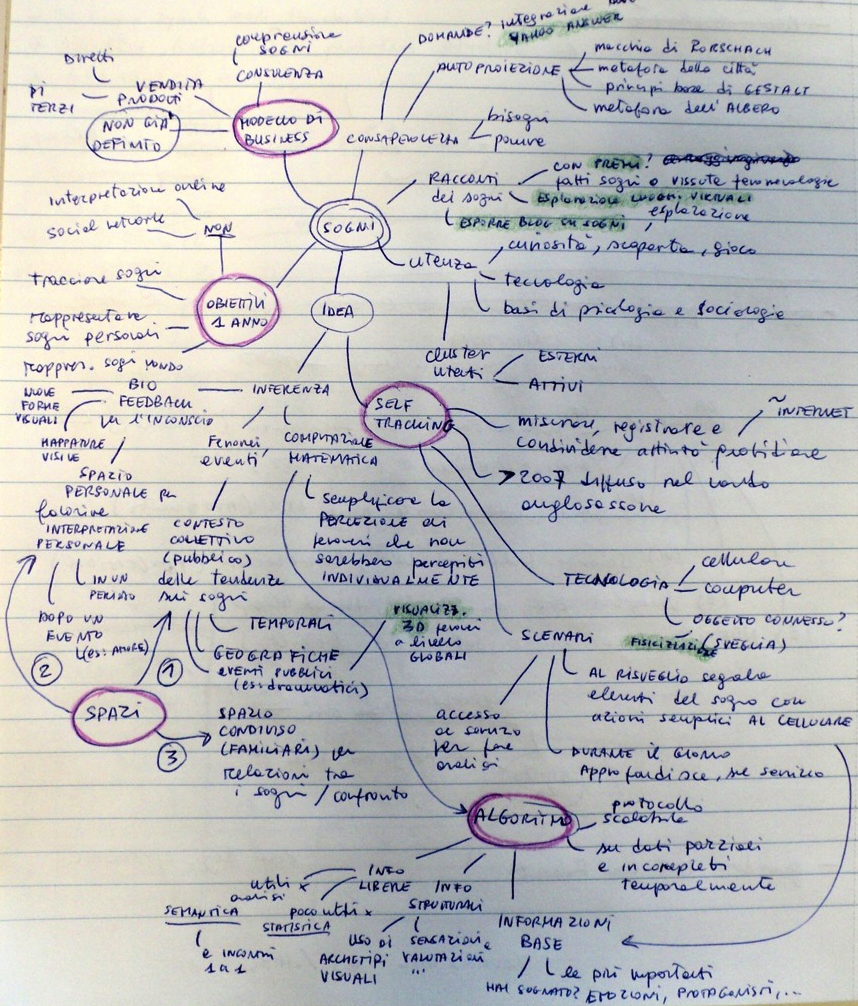
\includegraphics[scale=0.18]{images/mindmap.png}
		    \end{column}
		 \end{columns}
	\end{frame}

	\begin{frame}{Esplorazione: Cosa?}

		\begin{columns}[T]
		    \begin{column}{.5\textwidth}

				\begin{itemize}
					\item Storie, temi
					\item Scadenze, eventi
				\end{itemize}

				\begin{itemize}
					\item \textbf{Piano di Rilascio}
					\begin{itemize}
						\item Note, domande
						\item Nessuna stima
					\end{itemize}
					\item \textbf{Modello \\ del Dominio}
					\begin{itemize}
						\item Entità, relazioni
						\item Cardinalità
					\end{itemize}
				\end{itemize}
				
	    \end{column}
	    \begin{column}{.5\textwidth}
			\hspace*{-0.6cm}
		    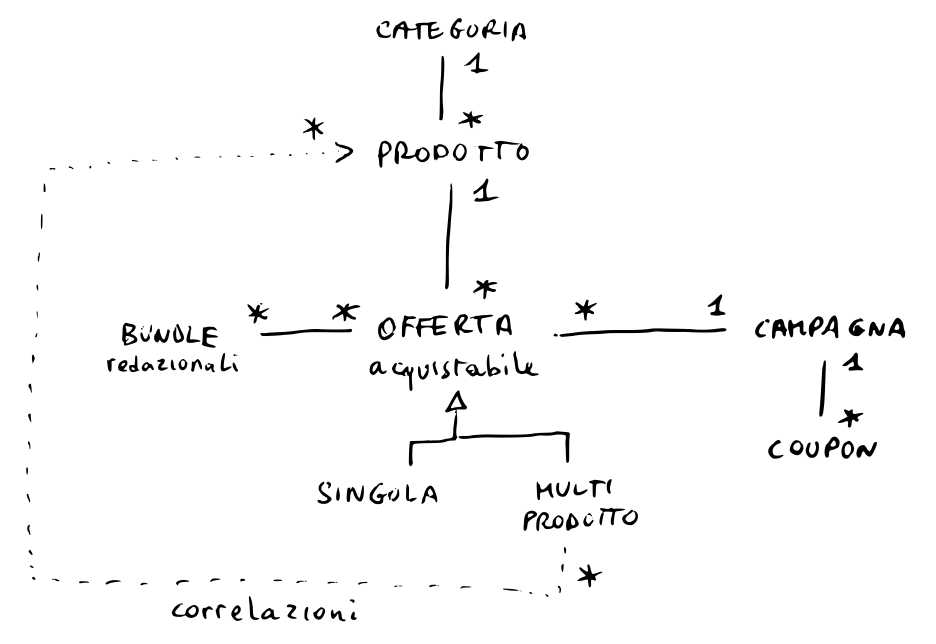
\includegraphics[scale=0.18]{images/domain.png}
	    \end{column}
	 \end{columns}
	\end{frame}

	\begin{frame}{Esplorazione: Come?}
		
		\begin{columns}[T]
		    \begin{column}{.5\textwidth}

		\begin{itemize}
			\item \textbf{Architettura Logica}
			\begin{itemize}
				\item Sistemi
				\item Interconnessioni
				\item Clients (e utenti)
			\end{itemize}
		\end{itemize}		
		
		\begin{itemize}
			\item Hosting
			\begin{itemize}
				\item In-house, cloud
				\item Pro, staging
			\end{itemize}
			\item Spikes
		\end{itemize}
		
	    \end{column}
	    \begin{column}{.5\textwidth}
			\hspace*{-0.6cm}
		    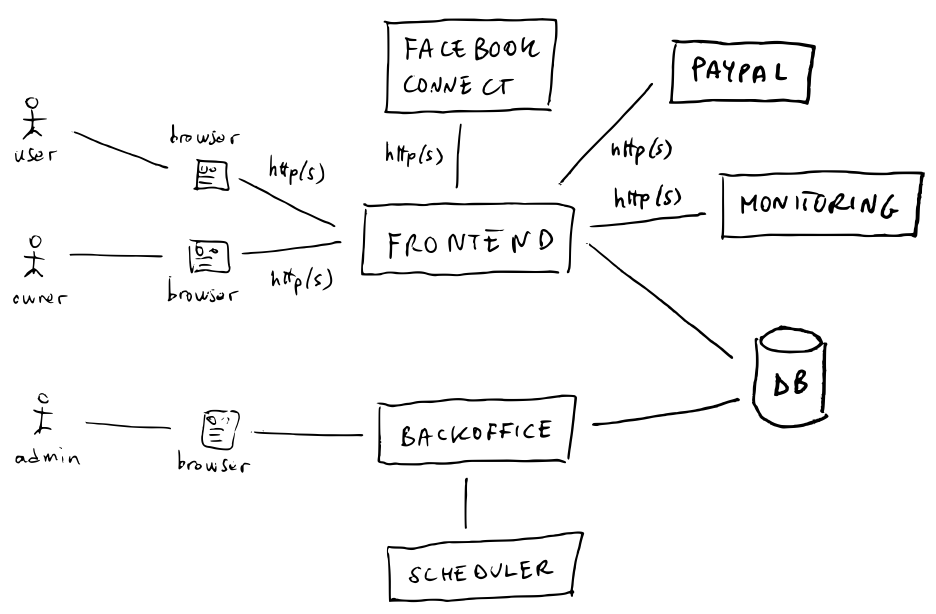
\includegraphics[scale=0.17]{images/architecture.png}
	    \end{column}
	 \end{columns}

	\end{frame}

	\begin{frame}{Commitment: Stima}
		
		\begin{columns}[T]
		    \begin{column}{.5\textwidth}
		
				\begin{itemize}
					\item Complessità
					\begin{itemize}
						\item Mimina, 50\%
						\item Massima, 90\%
						\item Giorni/coppia, settimane/coppia
					\end{itemize}
					\item Incertezza
					\begin{itemize}
						\item Buffer da stddev
					\end{itemize}
				\end{itemize}

				\begin{itemize}
					\item \textbf{Effort}
					\begin{itemize}
						\item 50\% + buffer
					\end{itemize}
				\end{itemize}
		
		    \end{column}
		    \begin{column}{.5\textwidth}
				\hspace*{-0.6cm}
			    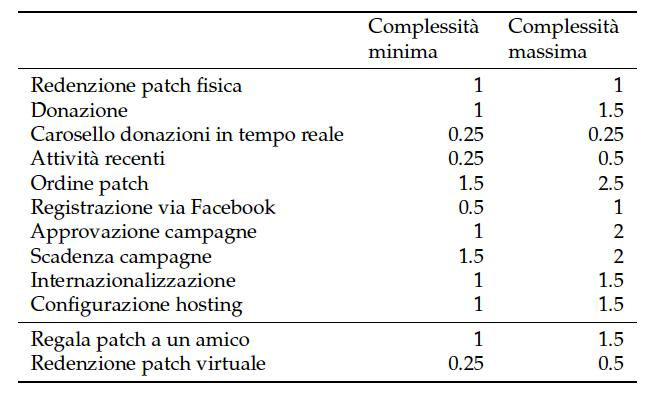
\includegraphics[scale=0.25]{images/estimates.png}
		    \end{column}
		 \end{columns}
	
	\end{frame}

	\begin{frame}{Commitment: Piano di Rilascio}
		\begin{itemize}
			\item Composizione team
		\end{itemize}

		\begin{itemize}
			\item \textbf{Elapsed}
		\end{itemize}
	\end{frame}
	
	\begin{frame}{Commitment: Economics}
		\begin{itemize}
			\item Sviluppo
			\item Hosting
			\item Servizi
		\end{itemize}

	\end{frame}
	
	\begin{frame}{Reporting}
		\begin{itemize}
			\item Introduzione
			\item Valutazione
			\begin{itemize}
				\item Modello del Dominio, Piano di Rilascio
				\item Tabelle riassuntive: Effort, Elapsed
			\end{itemize}
			\item Soluzione Tecnica
			\begin{itemize}
				\item Architettura Logica, Hosting
			\end{itemize}
			\item Economics
			\begin{itemize}
				\item Tabella riassuntiva: Costi
				\item Non un contratto!
			\end{itemize}
		\end{itemize}
	\end{frame}
	
	\begin{frame}{Sì, ma...}
		\begin{itemize}
			\item Ok per progetti di clienti, ma per \highlight{prodotti}?
			\item Chi \highlight{paga} per questa valutazione?
			\item E dopo? Il \highlight{contratto}? E il kick-off?
		\end{itemize}
		\begin{center}
			\hspace*{-0.6cm}
			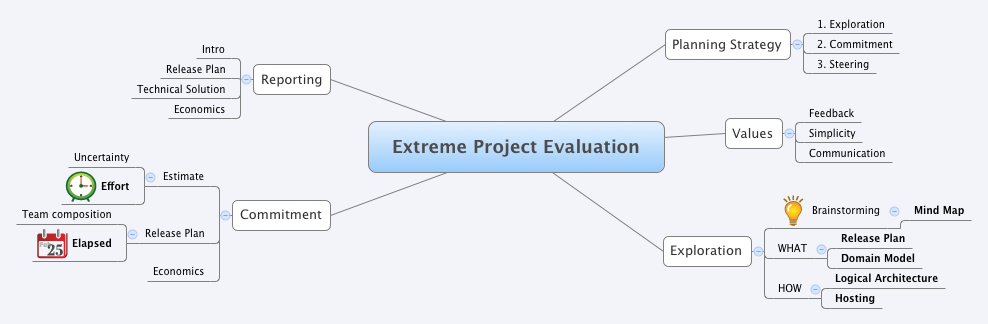
\includegraphics[scale=0.31]{images/takeaway.png}
		\end{center}
	\end{frame}
	
	\begin{frame}{Per Approfondire}
		\begin{itemize}
			\item {\small \highlight{Extreme Programming Explained - 1st ed}, K.Beck}
			\begin{itemize}
				\item Strategia di Pianificazione
				\item Valori
			\end{itemize}
			
			\item {\small \highlight{Agile Estimating and Planning}, M.Cohn}
			\begin{itemize}
				\item Incertezza nelle stime
			\end{itemize}
			
			\item {\footnotesize \highlight{\href{http://www.natpryce.com/articles/000755.html}{Test-Driven Development of Asynchronous Systems}}}{\small , N.Pryce}
				\begin{itemize}
					\item Architettura Logica
				\end{itemize}
		\end{itemize}
		
		\begin{itemize}
			\item Mind Mapping
			\item Reporting
			\begin{itemize}
				\item Text Processor: \highlight{LaTeX}
				\item VCS: \highlight{Subversion}, \highlight{Git}
			\end{itemize}
		\end{itemize}
	\end{frame}

\end{document}